\documentclass[11pt]{article}
\usepackage{authblk}
\usepackage{arydshln}
\usepackage[margin=2cm]{geometry}
\usepackage{adjustbox}
\usepackage{multirow}
\usepackage{arydshln}

\newcommand{\beginsupplement}{%
        \setcounter{table}{0}
        \renewcommand{\thetable}{S\arabic{table}}%
        \setcounter{figure}{0}
        \renewcommand{\thefigure}{S\arabic{figure}}%
     }
%\geometry{a4paper, portrait, margin=1.2in}

\setlength{\parskip}{\baselineskip}%
\setlength{\parindent}{30pt}%
\linespread{2}

\title{\textbf{Chapter 4:} Estimating the parameters of SSWs from patterns of genetic diversity in the house mouse genome}
\author[1,*]{Tom R. Booker}

\affil[1]{Institute of Evolutionary Biology, University of Edinburgh, Edinburgh}



\begin{document}
\maketitle
\begin{abstract}


\end{abstract}

%%%%%%%%%%%%%%%%%%%%%%%%%%%%%%%%%%%%%%%%%%%%%%%%%%%%
%
%  #   #    #  #####  #####  ######
%  #   ##   #    #    #   #  #    #     
%  #   # #  #    #    #####  #    #
%  #   #  # #    #    #  #   #    #           
%  #   #   ##    #    #   #  #    #  
%  #   #    #    #    #   #  ######    
%
%%%%%%%%%%%%%%%%%%%%%%%%%%%%%%%%%%%%%%%%%%%%%%%%%%%%
\section*{Introduction}

	Genetically linked sites do not evolve independently, so selection acting at one site may influence the fate of another. The consequences of selection at linked sites are intrinsically linked to the frequency and strength of selected mutations as well as, crucially, the rate of recombination \citep{RN124,RN206,RN287,RN157}. Two main modes of selection at linked sites have been identified; selective sweeps (SSWs) caused by the spread of advantageous mutations and background selection (BGS) caused by the removal of deleterious variants. The two processes are related and can both potentially explain the positive correlations between nucleotide diversity and recombination rate reported in many species \citep{RN117}. However, the proportion of nonsynonymous substitutions attributable to adaptive evolution ($\alpha$) is typically high (50\%) (\citealt{RN215}; but see \citealt{RN352} for caveats), suggesting that SSWs may play a substantial role in shaping nucleotide diversity across the genomes of many species.

	SSWs have been subject to rigorous population genetic research \citep{RN124, RN226, RN278, RN235}. The classic footprint of a selective sweep is a trough in nucleotide diversity at neutral sites surrounding substitutions. The reductions in nucleotide diversity caused by SSWs are related to the strength of selection acting on advantageous mutations as well as the frequency with which they arise. Taking advantage of this, \cite{RN277} used a model of SSWs to estimate the frequency and strength of advantageous mutations in \textit{Drosophila melanogaster} by fitting the positive correlation between recombination rate and nucleotide diversity. At the time of their analysis, the theory of BGS was in its infancy and models combining the effects of BGS and sweeps had not been developed. However, the effects of BGS are expected to be ubiquitous across the genome \citep{RN116, RN274, RN120}, and studies, conceptually similar to Wiehe and Stephan's (1993), have shown that controlling for BGS is highly important when parametrizing sweep models from patterns of nucleotide diversity \citep{RN290, RN274}.

	Both SSWs and BGS act to reduce nucleotide diversity, so it has proven difficult to distinguish their effects using population genetic data \citep{RN339}. A number of different approaches have been taken to tease apart the effects of the two processes. For instance, \cite{RN167} showed that, on average, there is a trough in diversity around recent nonsynonymous protein-coding substitutions in \textit{Drosophila melanogaster} but not around synonymous ones. This pattern is strongly suggestive of SSWs, so \cite{RN167} fitted a sweep model to the trough they observed and estimated that strongly advantageous mutations ($2N_es$ $\approx$ 5,000) occur in the fruitfly's genome.  In the house mouse, there is also a trough in diversity around recent nonsynonymous substitutions, but an almost identical trough is observed around synonymous substitutions, furthermore a similar trough is observed around even randomly selected synonymous and nonsynonymous sites in the genome \citep{RN122}. This all, perhaps, suggests that the reductions in diversity caused by selection at linked sites extend beyond the average distance separating nonsynonymous substitutions, so that the methods employed by \cite{RN167} are not effective in mice \citep{RN122}. However, values of $\alpha \geq 0.19$ have been reported for  multiple classes of functional elements \citep{RN122} and BGS alone cannot fully explain observed patterns of diversity (\citealt{RN122}, Chapter 3), suggesting that SSWs do contribute to the observed patterns in mice.

	In Chapter 3, we sought to tease apart the contribution of BGS and SSWs to patterns of diversity in mice. We estimated distributions of fitness effects (DFEs) for both harmful and advantageous mutations occurring in multiple classes of functional sites, analysing the distribution of derived allele frequencies (referred to as the unfolded site frequency spectrum, hereafter uSFS). The methods that we used, and related approaches, rely on the assumption that selected mutations segregate in populations of interest, such that they affect the shape of the uSFS. Using simulations, we found that neither BGS nor SSWs, given the selection parameters we estimated from the uSFS, could explain troughs in diversity observed around protein-coding exons and conserved non-coding elements (CNEs). A possible explanation for this finding is that advantageous mutations which have large effects on fitness, and which cause the greatest reduction in neutral diversity, may not be detectable by analysis of the uSFS. 

	In this study, we use a model of SSWs to estimate the strength and frequency of advantageous mutations that occur within protein-coding exons and regulatory elements. Using simulations, we show that the selection parameters that explain the troughs in diversity are out of the range detectable by analysis of the uSFS.  We find that the strength of selection acting on protein-coding exons is far greater than that acting in regulatory elements. Finally, using a simple model of the fitness change brought about by adaptive evolution, we show that, despite adaptation occurring more frequently in regulatory regions, adaptation in protein-coding regions may contribute more to phenotypic evolution in mice.

%%%%%%%%%%%%%%%%%%%%%%%%%%%%%%%%%%%%%%%%%%%%%%%%%%%%
%
% #   #  ####  #####  #   #  ####    ####
% ## ##  #       #    #   #  #   #   #  
% # # #  ###     #    #####  #   #   ####
% #   #  #       #    #   #  #   #      #        
% #   #  #       #    #   #  #   #      #
% #   #  ####    #    #   #  ####    ####
%
%%%%%%%%%%%%%%%%%%%%%%%%%%%%%%%%%%%%%%%%%%%%%%%%%%%%
\section*{Materials and Methods}

\subsection*{Model of SSWs with BGS}

	\cite{RN290} gave expressions for the neutral diversity expected under the combined effects of BGS (BGS) and SSWs (SSWs). They assumed that the effects of BGS and SSWs act independently so that their effects can simply be summed. However, BGS causes a reduction to the effective population size ($N_e$) at a neutral locus, $k$ by some fraction $B_k$, so may influence the rate and fixation probability of new advantageous mutations since both are dependant upon $N_e$. We scale the sweep effect by $B_k$ in a modified version of the model used by \cite{RN290},
	
\begin{equation}
\label{jointApprox}
\frac{\pi_{k}}{\pi_{0}} \approx  \frac{1}{B_{k}^{-1}  + B_{k}2N_eP_{sc,k}}.
\end{equation}

	Where $\pi_k$ is genetic diversity observed at neutral site \textit{k} and $\pi_0$ is diversity expected in the absence of selection at linked sites. $P_{sc,k}$ is the reduction in coalescence times at site $k$ caused by the effects of SSWs,

\begin{equation}
\label{singleClass}
P_{sc,k} \approx V_a \tau\gamma_a^{\frac{-4r_{i,k}}{s}} 
\end{equation}

The term $V_{a} = 2 \mu p_{a} \gamma_{a}$ is the rate of sweeps per base pair per generation, where $\mu$ is the point mutation rate, $p_a$ is the proportion of new mutations that are advantageous and $\gamma_a$ is the scaled selection coefficient ($2N_es_a$) of those mutations (Kimura and Ohta 1971). $\tau$ is the number of selected sites in a functional element and the recombination fraction between a functional element ($i$) and the focal neutral site is $r_{i,k}$. When assuming that recombination proceeds solely by crossing over $r_{i,k}$ is simply the product of the physical distance ($d_{i,k}$) and the local crossing-over rate ($r_c$). When incorporating gene conversion, we use Equation 1 from Frisse et al. (2001):
 		\begin{equation}
		\label{geneConversion}
		r_{i,k} = d_{i,k} r_c + g_c d_g \Bigg( 1 - e ^{-\frac{d_{i,k}}{d_g}} \Bigg)
		\end{equation} where $g_c$ is the rate of gene conversion and $d_g$ is the mean gene conversion tract length, assuming that the distribution of tract lengths is exponential. When applying Equation \ref{geneConversion} we use $g_c = \kappa r_c$ where $\kappa$ is the ratio of the non-crossovers to crossovers.
	
	Both theoretical and experimental results suggest that the distribution of fitness effects for advantageous mutations is exponential \citep{RN109}. We incorporate an exponential distribution of advantageous mutation effects to Equation 3 as follows:
		\begin{equation}
		\label{exponential}
P_{sc,k} \approx \int \limits_{0}^{\infty} f(\gamma) V_a \tau\gamma_a^{\frac{-4r_{i,k}}{s}} \mathop{d\gamma}
		\end{equation}

	
	We estimated $\gamma_a$ and $p_a$ by fitting Equation \ref{jointApprox} to the relationship between nucleotide diversity and genetic distance to functional elements using non-linear least squares with the \emph{lmfit} (0.9.7) package for Python 2.7. When analysing the mouse data, see below, we compared the fit of Equation \ref{jointApprox} incorporating either one or two discrete classes of advantageous mutations (Equation \ref{singleClass}) or the exponential distribution (Equation \ref{exponential}) using Aikieke's Information Criterion (AIC).
	
	\subsection*{Analysis of Mouse Data}

	We analysed patterns of genetic diversity present in 10 wild-caught \textit{M. m. castaneus} individuals, first reported by \cite{RN122}. Briefly, \cite{RN122} sequenced individual genomes to high coverage ($\approx$ 30x) using Illumina paired-end reads, which were then mapped to the mm9 mouse reference genome using BWA. Variants were called using a Samtools pipeline. Note that we only analyse SNP data in this study, insertion/deletion variants are not included. For further details of the sequencing and variant calling methods see \cite{RN122}. Protein-coding exons present in version 67 of the Ensembl annotation database and the locations of conserved non-coding elements (CNEs) identified by \cite{RN122} using an alignment of placental mammals were used in this study. The mean length of a protein-coding exon is 151bp, of which we assume 75\% of sites are subject to selection and the mean length of a conserved non-coding element is 51bp, of which 100\% of sites are subject to selection.

	From the edges of exons (CNEs), polymorphism data and divergence to the rn4 rat reference genome were extracted for non-CpG sites in windows of 1Kbp (100bp) extending to distances of 100Kbp (5Kbp). Analysis windows were then binned based on genetic distance to the focal element. Genetic distances were calculated using either the LD-based recombination map for \textit{M. m. castaneus} constructed by \cite{RN340} or the pedigree-based genetic map constructed using common lab strains of \textit{M. musculus} by \cite{RN232}. Because LD-based and pedigree-based recombination maps have different benefits and drawbacks (\textit{see Results}), we performed analyses based on both of these maps in parallel. Genetic distances calculated using the \cite{RN232} map were scaled assuming an $N_e$ of 426,200.

	Compared to crossing-over rates, gene conversion parameters are very difficult to estimate \citep{RN247}. Empirical estimates of the ratio of crossovers to non-crossovers (a parameter we have termed $\kappa$) vary across orders of magnitude in mammals \citep{RN247}. \cite{RN263} measured non-crossover gene conversion rates in three recombination hotspots in mice and estimated a mean gene conversion tract length of 144bp and $\kappa = 0.105$, we refer to this estimate as the low gene conversion rate. Values of $\kappa$ as high as 12.0 have been reported in humans (Paigen and Petkov 2010), so to explore the effects of high gene conversion rates on the parameters of SSWs inferred from models of selection at linked sites, we also assumed $\kappa$ = 12.0, which we refer to as the high gene conversion rate. 

	In order to disentangle the sweep parameters we obtained, we assume a point mutation rate of $5.4 \times 10^{-9}$, which is based on a mutation-accumulation experiment in \textit{M. musculus} \citep{RN228}.	We also assume an $N_e$ for \textit{M. m. castaneus} of 426,200, based upon the level at which diversity plateaus in the regions surrounding CNEs.

	\subsection*{Estimates of \textit{B}} 
 
 	BGS contributes to the troughs in diversity around both protein-coding exons and CNEs (\citealt{RN122}; Chapter 3). Because of this, we required estimates of the effect of BGS on neutral diversity, \textit{B}, to fit as a covariate when fitting Equation \ref{jointApprox} to diversity troughs. There are formulae for calculating \textit{B} given the DFE as well as mutation and recombination rates \citep{RN157, RN206}, but these over-predict the effects of BGS when purifying selection is weak ($\gamma_d < 1$) (Good and Desai 2014; Gordo et al. 2002). Since weakly deleterious mutations comprise a large portion of the DFEs previously obtained for mice (\citealt{RN122}, Chapter 3), we opted to obtain estimates of \textit{B} from simulations. In Chapter 3, we used simulations to estimate the contribution of BGS to patterns of nucleotide diversity around both protein-coding exons and CNEs. These simulations incorporated recombination rate variation, the actual distribution of functional elements in the genome and dDFEs specific to each of the functional elements analysed. By extracting $\frac{\pi}{\pi_0}$ as a function of genetic distance to both protein-coding exons and CNEs from these simulated data, we obtained estimates of \textit{B} that can be used when fitting Equation \ref{jointApprox}.
 	
 	The simulations we used to estimate $B$ were the same as those we used in Chapter 3, except that we increased the number of simulation replicates from 2,000 to 6,000. To obtain smoothed $B$ values we fit Loess curves to the simulation data using R (v3.4.2) using a span of 0.2 and using the number of sites contributing to each analysis bin as weights.

	\subsection*{Simulating the unfolded site frequency spectra}
	
	In Chapter 3 of this thesis, we argued that strongly selected advantageous mutations are difficult to detect by analysis of the uSFS. To these this hypothesis, we generated simulated datasets using the forward-time simulation package SLiM (v1.8; \citealt{RN148}). We simulated the evolution of 1Mbp chromosomes containing 20 evenly spaced out `genes`. Each `gene` consisted of 10 100bp exons, separated by 1Kbp of neutrally evolving intronic sequence. Nonsynonymous mutations were modelled as 75\% of mutations occurring in exons, the remaining 25\% were strictly neutral (i.e. synonymous sites). We varied the $\gamma_a$ and $p_a$ parameters across simulations, but kept the product $\gamma_a p_a$ equal to 0.1. We based this value of $\gamma_a p_a \approx 0.1$ on a recent study in \textit{D. melanogaster} \citep{RN321}. All simulations incorporated the same gamma dDFE (shape parameter $\beta$ = 0.2 and mean $\hat{\gamma_d}$ = -1,000), but the advantageous mutation parameters varied, these are listed in Table \ref{tab:advMuts}. The population-scaled mutation and recombination rates (i.e. $\theta$ = \emph{$4N_{e}\mu$} and $\rho$ = \emph{$4N_{e}r$}, respectively) were set to 0.01. Populations of $N$ = 1,000 diploid individuals were simulated for an initial burn-in of 10$N$ generations to establish equilibrium conditions. After the burn-in, 20 haploid chromosomes were sampled every 2$N$ generations for a further 100$N$ generations. We performed 10 replicate simulations for each set of selection parameters (Table \ref{tab:advMuts}). Across simulation replicates, time-points and loci we extracted the simulated nonsynonymous and synonymous sites, giving uSFS data for 10,000 `genes'. We sampled the set of 10,000 `genes' with replacement 100 times, collating the nonsynonymous and synonymous site uSFSs for each replicate.
	
	We estimated our simulated DFEs by analysis of the uSFS using the methods of \cite{RN354}, as implemented in the polyDFE (v1.1) package. polyDFE fits an expression for the uSFS expected in the presence of both advantageous and deleterious mutations to data from putatively neutral and selected classes of sites, and estimates parameters by maximum likelihood. The neutral class is used to determine distortions to the uSFS caused by processes such as selection at linked sites and a history of population size change. In addition, polyDFE corrects for polymorphism misattributed to divergence, mutation rate variability and error in assigning sites as ancestral/derived. \cite{RN354} performed extensive simulations and showed that accurate estimates of the parameters for both deleterious and advantageous mutations can be obtained using their methods. However, there are a range of parameters that they did not test which may be biologically relevant, specifically when advantageous mutations are strongly selected, but infrequent.

	 We analysed the simulated uSFS data using polyDFE choosing Model C (a gamma dDFE and a discrete class of advantageous mutations) and either including or not between-species divergence. We analysed the uSFS for simulated nonsynonymous sites using synonymous sites as the neutral reference class. For each of the advantageous mutation parameter sets tested, we analysed 100 bootstrap samples of the simulation data.
 
 	
%%%%%%%%%%%%%%%%%%%%%%%%%%%%%%%%%%%%%%%%%%%%%%%%%%%%
%
% ####   ####  #####  #   #  #     #######  #####
% #   #  #     #      #   #  #        #     #
% ## #   ###   #####  #   #  #        #     #####
% # #    #         #  #   #  #        #         #
% #  #   #         #  #   #  #        #         #
% #   #  ####  #####  #####  #####    #     #####
%
%%%%%%%%%%%%%%%%%%%%%%%%%%%%%%%%%%%%%%%%%%%%%%%%%%%%


\section*{Results}

\subsection*{Patterns of genetic diversity around protein-coding exons and conserved non-coding elements}

\begin{figure}[h]
   \centering      
   \noindent\makebox[\textwidth]{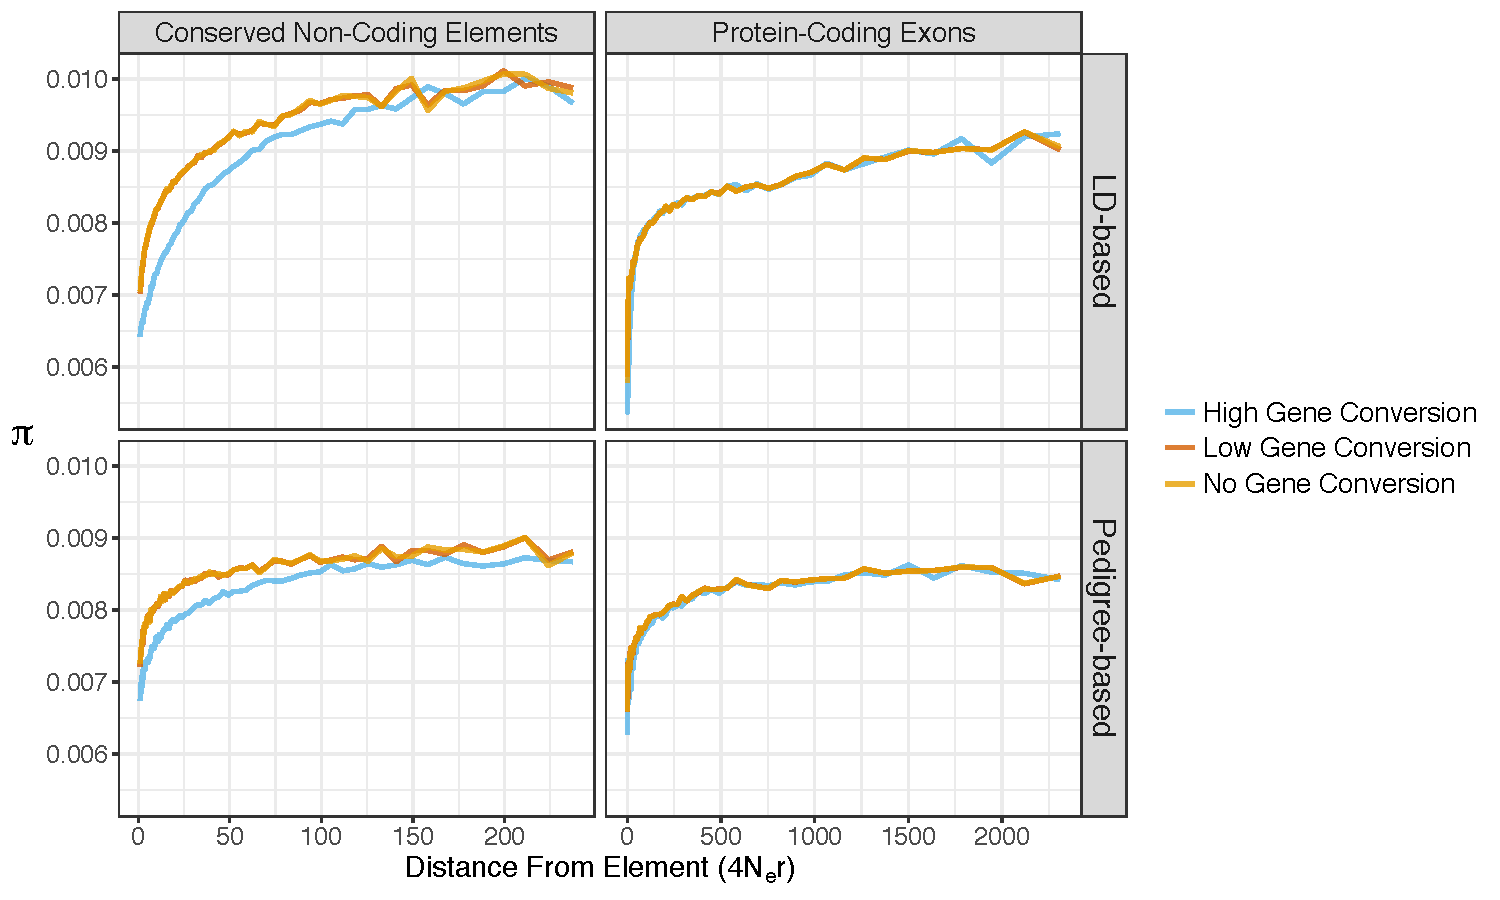
\includegraphics[width=\textwidth]{/Users/s0784966/PhD/Coding/Estimate_selection_from_troughs/report/figures/Pi_geneticDistance_4x4.pdf}}
 \caption{Nucleotide diversity in regions surrounding protein-coding exons and conserved non-coding elements in wild mice. Population-scaled genetic distances($4N_er$) were calculated using either an LD-based recombination map constructed for \textit{M. m. castaneus} or the pedigree based \textit{M. musculus} genetic map constructed by \cite{RN232}. Gene conversion was included assuming either the gene conversion rates }.
 
 \label{fig:Diversity2x2}
\end{figure}

\linespread{1}
\begin{figure}[h]
   \centering      
   \noindent\makebox[\textwidth]{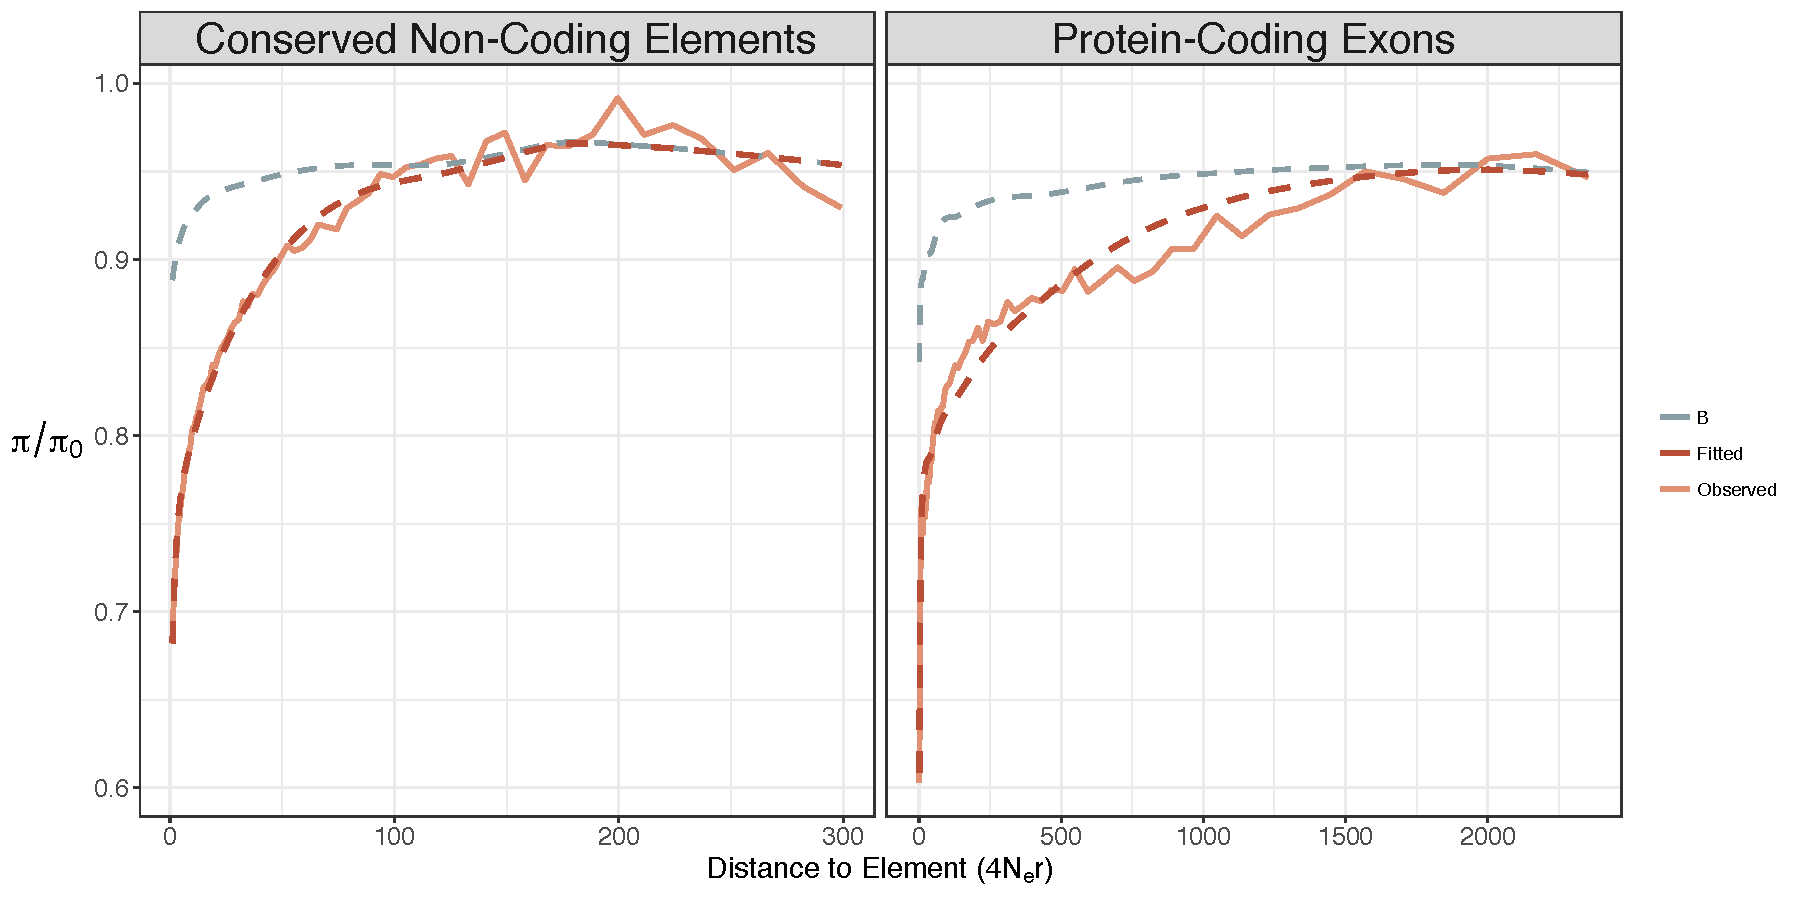
\includegraphics[width=\textwidth]{/Users/s0784966/PhD/Coding/Estimate_selection_from_troughs/mouse_analysis/ModelFit.pdf}}
 \caption{The pattern of scaled nucleotide diversity around protein-coding exons and CNEs in \textit{M. m. castaneus}.}  
 
 \label{fig:castaneusFit}
\end{figure}

	Recombination rates can be estimated in various ways, which have different pros and cons. For instance, the population-scaled recombination rate ($\rho$) can be inferred from a relatively small sample of unrelated individuals at very fine-scales using patterns of linkage disequilibrium (LD). However, selection at linked sites influences local LD and may therefore affect recombination rate estimates obtained in this way (Clark REVIEW). Alternatively, direct estimates of the recombination rate ($r$) can be obtained from crossing experiments, but to achieve sufficient power to generate recombination maps a very large number of individuals need to be genotyped, which has typically precluded the use of whole-genome re-sequencing, limiting resolution. In summary, high resolution recombination maps can be generated using patterns of LD, but these may be biased by selection at linked sites, while unbiased recombination maps may be generated using crosses, though these typically have low resolution. When analysing patterns of genetic diversity using a model of selection at linked sites, the way in which recombination rate estimates were obtained may, therefore, affect parameter estimates.

	In this study, we analysed the relationship between nucleotide diversity and genetic distances from funcitonal eleemnts in \textit{M. m. castaneus} assuming either the high resolution recombination map constructed from LD by \cite{RN340} (the \textit{castaneus} map) or the pedigree-based map of \cite{RN232} (the Cox map). The choice of recombination map had a substantial effect on patterns of nucleotide diversity. We found that, in the immediate flanks of both exons and CNEs, diversity was lower when assuming the LD-based \textit{castaneus} map than when assuming the pedigree-based Cox map (Figure \ref{fig:Diversity2x2}). This difference is consistent with the idea that regions of the genome close to functional elements, where the effects of BGS and/or SSWs are strongest, and thus exhibit reduced diversity, may yield downwardly biased estimates of the recombination rate obtained from LD. An alternative explanation is that the Cox map, which lacks resolution, does not fully capture regions of low recombination rate, causing analysis windows that are tightly linked to functional elements to appear less tightly linked. However, genetic diversity  plateaus at a higher level when assuming the \textit{castaneus} map, suggesting that the Cox map may not capture some of the highly recombining portions of the genome. The choice of recombination map will, therefore, have an impact on the parameters of selection inferred from the patterns of diversity. Throughout the rest of this chapter, we present, in parallel, the results of analyses based on the \textit{castaneus} map with those based on the Cox map.

	\subsection*{Diversity expected in the absence of selection, $\pi_0$}

	A key parameter in Equation \ref{jointApprox} is $\pi_0$, the nucleotide diversity expected in the absence of the effects of selection at linked sites. This parameter is very difficult to estimate and may even prove unobservable in real data given the ubiquity of the effects of selection at linked sites \citep{RN357}, yet it is required. One strategy for estimating $\pi_0$ would be to divide the mean $\pi$ in regions sufficiently distant to functional elements by the corresponding value of $B$. $B$ plateaus at approximately 0.95 in regions surrounding both protein-coding exons and CNEs, but the level at which observed diversity plateaus is different for the two classes of elements (Figure), so it may be that SSWs at elements linked to exons have reduced overall diversity more than for CNEs. Simply dividing observed $\pi$ by $B$, would therefore give an underestimate of $\pi_0$ as does not incorporate the reduction in diversity caused by SSWs at linked elements. 	When analysing patterns of diversity around protein-coding exons, we assumed $pi_0$ values of 0.00955 and 0.00895 when using the \textit{castaneus} and Cox maps, respectively. When analysing patterns of diversity around CNEs, we assumed $pi_0$ values of 0.0102 and 0.00915 when using the \textit{castaneus} and Cox maps, respectively. 
	
\subsection*{Parameters of selective sweep obtained from patterns of nucleotide diversity}

	When fitting a model of SSWs and BGS to the reductions in diversity around exons and CNEs, we found that a two classes of advantageous mutational effects typically gave a substantially better fit to the data than did a single class or an exponential distribution (as judged by AIC). This result held regardless of the recombination map assumed and whether or not gene conversion was included in the analysis. The only exception was that an exponential distribution gave the best fit when protein-coding exons were analysed using the \textit{castaneus} map and the high gene conversion rate was assumed, but in this case the difference in fit was fairly small (Table X).
	
	For both protein-coding exons and CNEs we estimated a class of strongly advantageous mutations and a class of more weakly selected mutations (Table \ref{EstimatesCastaneus}). When assuming the \textit{castaneus} map and the low gene conversion rate, we estimated advantageous mutations with scaled effects ($\gamma_a$) of 8,470 and 432 for protein-coding exons and CNEs, respectively. The frequencies of these mutations were substantially different between the site classes
	For both classes of sites, we inferred a class of more frequent, more mildly advantageous mutations as well.
	
	inferred positively selected mutations with large fitness. We estimated stpositively selected mutations with $\gamma_a$ = 8,470 and 

	Ignoring the contribution of BGS by setting $B$ to 1.0 when fitting Equation \ref{jointApprox} to the diversity troughs resulted in a much poorer model fit (Table \ref{tab:BGSeffect}). The strength of selection acting on advantageous mutations estimated when ignoring BGS is far greater than when BGS is accounted for. This is presumable because selection 
	strength of selection acting on advantageous mutations was estimated to be higher and the frequency lower when BGS was ignored, for both classes of elements, for both recombination maps (Table \ref{tab:BGSeffect}). 
	
	In the absence of BGS effects, the strength of advantageous mutations required to explain the observed data is more far higher (Table \ref{tab:BGSeffect}), consistant with \cite{RN290}. Furthermore, ignoring the contribution of BGS by setting $B$ to 1.0 when fitting Equation \ref{jointApprox} to the diversity troughs resulted in a much poorer model fit.  
	
	The gene conversion parameters of Paigen \textit{et al} did not substantially influence the analysis.
	



\begin{table}[h]
\caption{Estimates of the DFE obtained from troughs in diversity around functional elements. Standard errors are shown in square brackets}
\centering

        \begin{tabular}{cccccc}

        \hline
             \multirow{2}{*}{BGS}& \multirow{2}{*}{Gene Conversion} & \multicolumn{2}{c}{Protein-Coding Exons} & \multicolumn{2}{c}{Conserved Non-Coding Elements}  \\
 & & $\gamma_a$ & $p_a$ &$\gamma_a$ & $p_a$  \\ [0.5ex] \hline
 
 \multirow{2}{*}{+} & \multirow{2}{*}{+} & & & &  \\
   &  &  [ ]& []& [  ] & []\\ \hdashline
 
 \multirow{2}{*}{-} & \multirow{2}{*}{+} &   &  & & \\
   &  &  []& []& [] & []\\ \hdashline

 \multirow{2}{*}{+} & \multirow{2}{*}{-} &  8,350 & 1.29 x $10^{-5}$ & 228 & 2.27 x $10^{-3}$ \\
   &  &  [ 1,680 ]& [ 4.23 x $10^{-6}$ ]& [ 12.8 ] & [2.40 x $10^{-4}$ ]\\ \hdashline
   
 \multirow{2}{*}{-} & \multirow{2}{*}{-} &  20,200 & 8.61 x $10^{-6}$ & 504 & 1.27 x $10^{-3}$ \\
  &  & [ 1,460 ] & [ 9.52 x $10^{-7}$ ]& [ 18.2 ] & [ 7.12 x $10^{-5}$ ]\\ \hline

        \end{tabular}
    \label{tab:Table1}
    
\end{table}




\begin{sidewaystable}
\caption{Positive selection parameter estimates obtained by analysis of the uSFS for simulated poplations. }
\begin{tabular}{ccccccc}

\toprule
 \multirow{2}{*}{Divergence \footnote{+/- indicates whether or not divergence was included when analysing the uSFS} } & \multicolumn{2}{c}{$\gamma_a$} & \multicolumn{2}{c}{$p_a$}  & \multirow{2}{*}{$\gamma_a p_a$} & Prop.\\
 	&    \textit{Simulated} & \textit{Estimated} & \textit{Simulated} & \textit{Estimated} &  &  Significant \footnote{The proportion of bootstrap replicates where a full DFE gave a significantly better fit than a model containing just deleterious mutations}\\
\midrule
         + &    \multirow{2}{*}{10} & 11.2 [5.60 - 20.0] &  \multirow{2}{*}{0.010000} & 0.00856 [0.00440 - 0.0199] &  0.0954 [0.0838 - 0.115] &  1.00 \\
         - &     & 3.97 [1.13 - 27.2] &   &         0.0201 [0.00472 - 0.0706] &  0.0828 [0.0616 - 0.155] &               1.00 \\
         + &   \multirow{2}{*}{20} &           16.6 [9.20 - 37.4] &  \multirow{2}{*}{0.005000} &  0.00568 [0.00241 - 0.0107] &  0.0949 [0.0822 - 0.108] & 1.00 \\
         - &    &        19.9 [2.90 - 37.4] &   & 0.00532 [0.00289 - 0.0207] &  0.106 [0.0454 - 0.193] &  0.97 \\
         + &   \multirow{2}{*}{50} &   37.4 [21.6 - 41.8] &  \multirow{2}{*}{0.002000} & 0.00257 [0.00202 - 0.00467] &  0.0951 [0.0809 - 0.106] & 1.00 \\
         - &    &   37.3[1.87 - 65.5] &  & 0.00266 [0.00125 - 0.0146] &  0.0717 [0.0112 - 0.145] &  0.86 \\
         + &   \multirow{2}{*}{100} &   37.43 [37.4 - 1530] &  \multirow{2}{*}{0.001000} &        0.00249 [0.0000738 - 0.00283] &   0.0938 [0.0795 - 0.107] &  1.00 \\
         - &    &  0.323 [0.0371 - 1.25] &   &  0.00259 [0.000525 - 0.0941] &  0.00102 [0.0000620 - 0.0137] & 0.00 \\
         + &  \multirow{2}{*}{200} &  37.4 [37.4 - 1,700] &  \multirow{2}{*}{0.000500} & 0.00251 [0.000220 - 0.00283] &     0.0947 [0.0738 - 0.106] & 1.00 \\
         - &   &            0.272 [0.00546 - 1.911] &   &                     0.0122 [0.000690 - 0.138] &  0.00310 [0.000104 - 0.0294] & 0.07 \\
         + &  \multirow{2}{*}{400} & 37.4 [32.7 - 37.4] &  \multirow{2}{*}{0.000250} & 0.00245 [0.00199 - 0.00283] &  0.0919 [0.0776 - 0.102] & 1.00 \\
         - &   & 12.3 [0.287 - 66.6] &   &  0.00212 [0.000783 - 0.0104] &  0.0338 [0.000250 - 0.0984] & 0.22 \\
         + &  \multirow{2}{*}{800} & 37.4 [32.9 - 37.4] &  \multirow{2}{*}{0.000125} & 0.00222 [0.00186 - 0.00264] &       0.0831 [0.0701 - 0.0936] & 1.00 \\
         - &   & 1.75 [0.111 - 43.0] &   &  0.00240 [0.000343 - 0.0293] &  0.0134 [0.0000515 - 0.0649] & 0.12 \\
\bottomrule
\end{tabular}
  \label{tab:advMuts}

\end{sidewaystable}

\subsection*{Estimating selection parameters from the uSFS of simulated data}

\linespread{1}

\begin{figure}[h]
   \centering      
   \noindent\makebox[\textwidth]{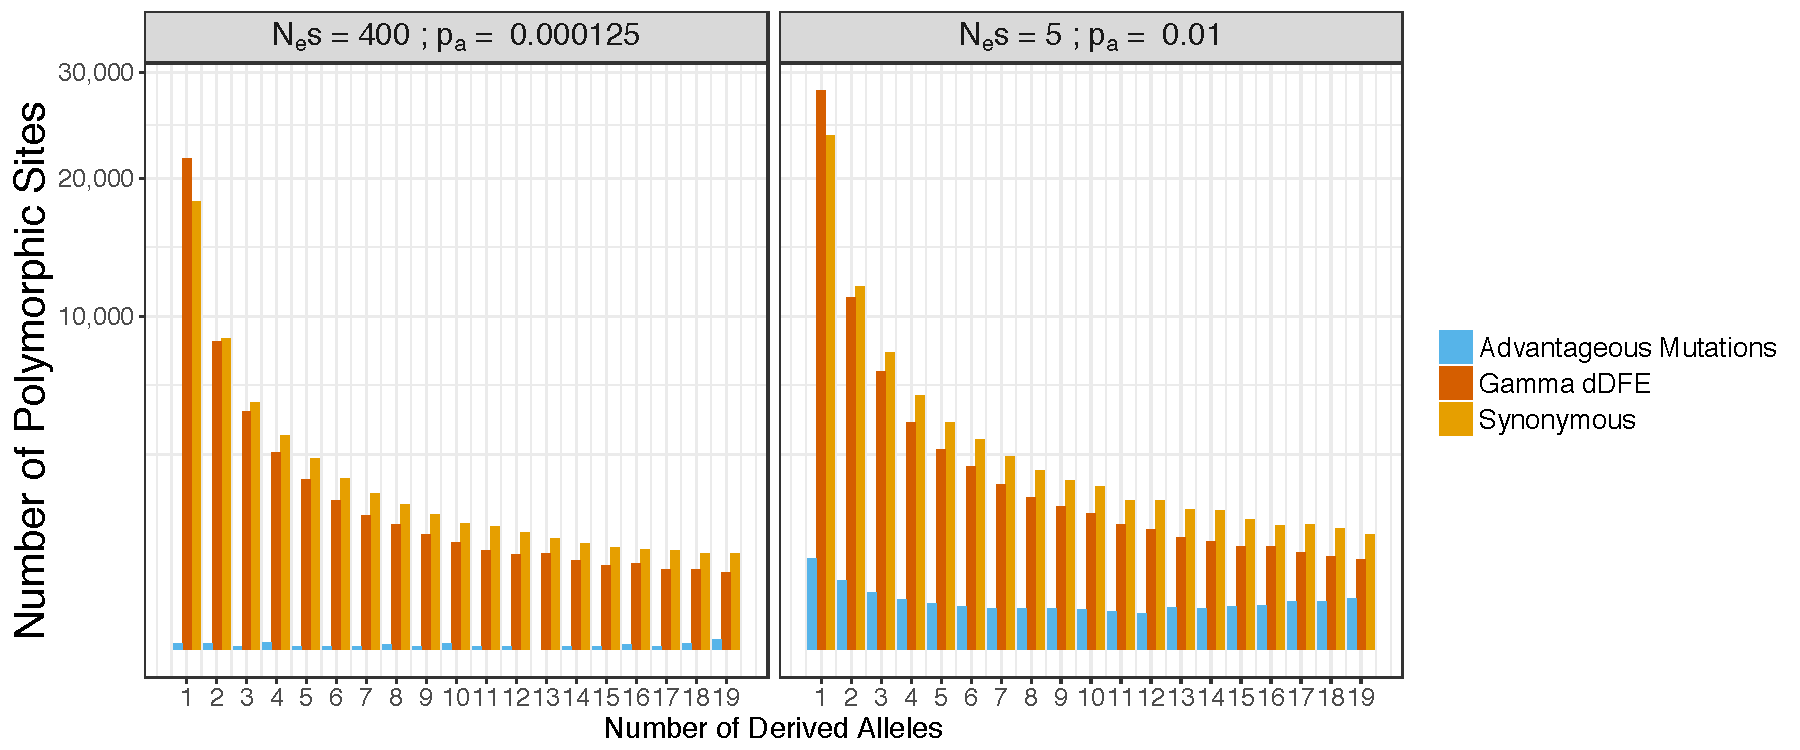
\includegraphics[width=\textwidth]{/Users/s0784966/PhD/Coding/Estimate_selection_from_troughs/simulations/NewSimulations/SFSplot/SFSplot.pdf}}
 \caption{An example of the uSFSs for deleterious (Gamma dDFE) and advantageous nonsynonymous sites with neutral synonymous sites from simulated populations. Results shown are from simulations modelling strongly or weakly advantageous mutations. The uSFS  model the same rate of synonymous substitutions $\gamma_a p_a = 0.1$. Simulated datasets included 10Mbp of exonic sites (3:1 nonsynonymous:synonymous sites).}
 
 \label{fig:sfsExample}
\end{figure}
\linespread{1}

	Parameters of the DFE can be estimated directly from polymorphism data if selected mutations are segregating in populations of interest (\textit{Reviewed in} \citealt{RN109}). It has been repeatedly demonstrated that parameters of the DFE for deleterious mutations (dDFE) can be accurately estimated from the SFS \citep{RN201, RN164, RN178, RN354}. It has also been shown that the parameters of advantageous mutations can also be estimated from the uSFS \citep{RN210, RN354}, but it has been argued that strongly selected advantageous mutations, which may contribute little to standing variation, will be undetectable by such methods (\citealt{RN290}; Chapter 3). In this study, we confirm this verbal argument using simulations, showing that accurate estimation of positive selection parameters does indeed depend on the strength and relative frequencies of advantageous mutations. We used forward-in-time simulations that incorporated linkage, because selection at linked sites can distort the uSFS in ways that likely affect real data and thus cannot be ignored. For each set of advantageous mutation parameters, we simulated 10Mbp of gene-like sequences giving a total of 7.5Mbp of nonsynonymous sites and 2.5Mbp of synonymous sites which we used to construct the uSFS for 20 haploid individuals. This sample size and quantity of data is fairly typical of population genomic datasets (e.g. \citealt{RN236, RN238, RN368}). 

	Across simulations, the strength of selection differed (ranging between $\gamma_a$ = 10 and $\gamma_a$ = 800), but the product $\gamma_a p_a$, which is expected to be directly proportional to the rate of sweeps, was always equal to 0.1. All simulations were subject to the same dDFE, so the extent of BGS should be fairly similar. We found that selection at linked sites reduced synonymous site diversity below the expectation value of 0.01 in all simulations (Table \ref{tab:summaryStats}),  but as the strength of selection acting on advantageous mutations increased, diversity at linked sites decreased (reflected in in the decreasing values $\pi/\pi_0$ shown in Table \ref{tab:summaryStats}). As expected, the relative fixation rate of nonsynonymous mutations (meausured using  $dN/dS$ ) did not vary systematically across simulations (Table \ref{tab:summaryStats}). From a visual inspection of the frequency spectra, it is clear that there is little information in standing variation for inferring the positive selection parameters when selection is strong (Figure \ref{fig:sfsExample}).
	

\begin{table}
\label{tab:summaryStats}
   \centering
   \begin{threeparttable}[b]
\caption{Summary statistics for simulated populations}

\begin{tabular}{cccccc}
\toprule
 $\gamma_a$ &       $p_a$ &   $\pi / \pi_0$ &        $dS$ &        $dN$ &     $dN/dS$ \\
\midrule
       5 &  0.010000 &  0.940 &  0.00533 &  0.00159 &  0.299 \\
      10 &  0.005000 &  0.914 &  0.00526 &  0.00157 &  0.299 \\
      25 &  0.002000 &  0.880 &  0.00527 &  0.00159 &  0.302 \\
      50 &  0.001000 &  0.862 &  0.00525 &  0.00162 &  0.309 \\
     100 &  0.000500 &  0.844 &  0.00531 &  0.00159 &  0.300 \\
     200 &  0.000250 &  0.819 &  0.00523 &  0.00155 &  0.296 \\
     400 &  0.000125 &  0.795 &  0.00527 &  0.00156 &  0.295 \\
\bottomrule
\end{tabular}

   \end{threeparttable}

   \end{table}
	
	
	 We analysed the uSFS from our simulated populations and found that when advantageous mutations are relatively frequent ($p_a$ $>$ 0.0005), but weakly selected ($\gamma_a$ $<$ 100), both $\gamma_a$ and $p_a$ parameters can be estimated with precision (Table \ref{tab:Table2}). However, we found that when advantageous mutations were infrequent but strongly selected ($\gamma_a$ $\geq$ 100 and $p_a$ $\leq$ 0.0005) the parameters were very poorly estimated. Across all simulated datasets, when we included divergence in the analysis, the product $\gamma_a p_a$ was accurately estimated (Table REF) and likelihood ratio tests never failed to detect the presence of advantageous mutations in the uSFS. When we excluded divergence from the analysis, however, the product  $\gamma_a p_a$  was poorly estimated when $\gamma_a \geq 100$ and likelihood ratio tests typically failed to detect positive selection (Table REF). Across all simulations, we found that polyDFE gave estimates of the dDFE which were highly accurate (Table \ref{tab:dDFE}). polyDFE performed most poorly when divergence was included in the analysis, but only a dDFE was inferred. These results replicate the findings of \cite{RN354} and further emphasize the importance of specifying a full DFE model when making inferences of selection from the uSFS. 

%%%%%%%%%%%%%%%%%%%%%%%%%%%%%%%%%%%%%%%%%%%%%%%%%%%%
%
% ####  #  #####  #####  #   #    #####  #####
% #   # #  #      #      #   #    #      #
% #   # #  #####  #      #   #    #####  #####
% #   # #      #  #      #   #        #      #
% #   # #      #  #      #   #        #      #
% ####  #  #####  #####  #####    #####  #####
%
%%%%%%%%%%%%%%%%%%%%%%%%%%%%%%%%%%%%%%%%%%%%%%%%%%%%

\section*{Discussion}

	BGS and SSWs both operate in the mouse genome. By fitting a model combining the effects of both processes to the troughs in diversity around protein-coding exons and CNEs in \textit{M. m. castaneus}, we estimated parameters of positively selected mutations occurring in the two classes of element that predict the observed patterns. This relied on estimates of the reduction in diversity caused by BGS ($B$), which, in turn, relied on estimates of the DFE for harmful variants. The dDFE can be accurately estimated from the uSFS as long as the dDFE is estimated using a model that includes advantageous mutations (Table \ref{tab:dDFE}) \citep{RN354}. 

	Here we have estimated parameters of positive selection from patterns of genetic diversity in the house mouse genome. We found that protein-coding regions experience more strongly selected mutation than do conserved non-coding elements. For both classes of sites, we found statistical support for two classes of advantageous mutational effects, one strong ($\gamma_a > 200$) and one comparatively weak. Using simulations, we demonstrated that the parameter estimates that we obtained are likely out of the range detectable by analysis of the uSFS.
	
\subsection*{The relative contribution of adaptive substitutions in protein-coding and regulatory regions to fitness change in mice}

	An enduring goal of evolutionary biology has been to understand the extent to which protein-coding and regulatory regions of the genome contribute to phenotypic evolution \citep{RN347, RN346}. \cite{RN347} posited that, since identity between human and chimpanzee proteins is around 99\%, changes in gene regulation may explain the plethora of phenotypic differences between humans and chimps. Using a simple model of the fitness change brought about by the substitution of advantageous mutations, we can use the parameter estimates we obtained in this study to try and understand the contribution of protein-coding and regulatory regions of the genome make to phenotypic evolution.

	Consider the following model of the fitness change brought about by the fixation of advantageous mutations ($\Delta W$). New mutations occur at a particular class of sites with rate $\mu$ per base-pair, per generation. A proportion of these new mutations, $p_a$, are advantageous with an expected selection coefficient of $s_a$. The advantageous mutations fix with probability $u(s_a)$ and once fixed contribute $s_a$ to the change in fitness. If it is assumed that selection is strong relative to genetic drift, then $u(s_a)$ is approximately $s_a$, giving the following expression:

		\begin{equation}
		\label{eq:fitness}
		\Delta W \propto \mu p_a n_a E(s_a)^2,
		\end{equation}

	We parametrized Equation \ref{eq:fitness} using the estimates of selection we estimated in this study, summing the fitness contribution for the two classes of fitness effect. We assume that the average point mutation rate is the same for CNEs and protein-coding exons, so we ignore $\mu$ in Equation \ref{eq:fitness}. 
 
	Based on our parameter estimates, we find that adaptation is far more frequent in CNEs than it is in protein-coding exons, but that protein-coding regions contribute more to fitness change. We inferred that the proportion of mutations occurring in CNEs that are advantageous is more than an order of magnitude higher than for protein-coding exons. Because of this and the fact that there are about three times as many CNE bases in the genome as there are protein-coding sites, the rate of advantageous mutations occurring in CNEs likely exceeds the rate in protein-coding regions. However, the average strength of selection acting on a new advantageous mutation in a protein-coding exon far exceeds that of a mutation in a CNE (Table \ref{EstimatesCastaneus}) and since the change in adaptive fitness is dependant on the square of the selection coefficient (it is related to the additive genetic variance in fitness), the change in population mean fitness brought about by the fixation of advantageous mutations is higher for protein-coding exons than for CNEs (Table \ref{tab:fitnessTable}. The difference we found was small (around 3 times higher for protein-coding regions than for regulatory regions), but was robust to the choice of recombination map (Table REF).
	
%	\cite{RN346} argued that changes to regulatory regions will contribute more to the anatomical evolution than will protein-coding changes, based on the argument that pleitropy 
%	 and that may be the case. Our analysis distils a large amount of information down to a single point
	
%	 Furthermore, \cite{RN346} suggested that pleiotropy may place a burden on protein-coding genes such that adaptation most often occurs in regulatory regions. 

%


\begin{table}
\centering

\caption{Rough estimates of the changes in fitness caused by new mutations occuring in protein-coding exons and CNEs. Estimates were obtained assuming an effective population size of 420,000 and a per base-pair per generation mutation rate of 5.4 x $10^{-9}$ (Uchimura \textit{et al.} 2015).}
 \begin{tabular}{l c c c c} 

  \hline
		& $\mu_a$  & $n_a$ (x $10^6$)& $s_a^2$ & $\Delta W$ x ($10^{-12}$) \\ [0.5ex] \hline
	Exons & 6.70 x $10^{-14}$ & 24.0 & 1.39 x $10^{-4}$ & 224 \\
	CNEs  & 1.23 x $10^{-11}$ & 54.2 & 7.36 x $10^{-9}$ & 4.91 \\ \hline
\end{tabular}    
    \label{t}

\end{table}


	There are a number of factors that should, perhaps, temper these conclusions. Firstly, the selection coefficient that appears in Equation \ref{eq:fitness} is the expectation of the DFE for advantageous mutations. If there were a continuous distribution of $s$ values around the point estimates we obtained, integrating over this distribution may yield a different result. Secondly, we have assumed that all elements of a particular class share a common set of selection parameters. This is slightly problematic since there are a number of sub-categorisations that could be applied to the set of CNEs we analysed (e.g. promoters and enhancers may be subject to different selective pressures). Indeed, different categories of protein-coding genes may also be subject to different selection pressures. For instance, virus interacting proteins and highly expressed genes have been estimated to have higher rates of adaptive substitutions in different organisms (Enard eLife paper; Williamson).

	Whether or not the conclusions we have drawn in this study can be generalised to other organisms remains to be seen, but the brown rat, \textit{Rattus norvegicus}, provides a compelling first case for comparison. In \textit{R. norvegicus} there are troughs in nucleotide diversity around protein-coding exons and CNEs that are very similar to those observed in \textit{M. m. castaneus} \citep{RN327}. Since broad-scale recombination rates are similar in mice and rats \citep{RN184}, qualitatively similar conclusions regarding the contribution of protein-coding versus regulatory change to adaptive evolution may be reached when analysing patterns of genetic diversity in rats. 

\subsection*{Estimating parameters of positive selection from the uSFS versus patterns of diversity}

	By analysing the uSFS of simulated populations, polyDFE yielded accurate estimates of the dDFE from simulated data, even when positive selection was very strong. Analysing simulated uSFSs with polyDFE yielded estimates of the dDFE that were extremely precise, but this depended on whether or not divergence was included and whether a full DFE was inferred. This is particularly evident for the case when $\gamma_a$ = 10 and $p_a$ = 0.01 (Table \ref{tab:dDFE}), where advantageous mutations contribute substantially to both standing variation and between-species divergence (Figure \ref{fig:sfsExample}; Table \ref{tab:summaryStats}). In this case, by limiting the inference to just the dDFE, advantageous mutations that contribute to the shape of the uSFS are assumed to be deleterious, resulting in spurious dDFE inferences. In the simulations where $\gamma_a$ = 400 and $p_a$ 0.000125, advantageous mutations make little contribution to standing variation, and the effect of not modelling a full DFE is less pronounced (Table \ref{tab:dDFE}).

	The number of fixed, advantageous mutations carries information on the compound parameter $\gamma_a p_a$ (Kimura and Ohta 1971), which will be embedded within between species divergence at selected sites. When there is little information present in the polymorphism data, this compound parameter cannot be further disentangled. Increasing the strength of selection, but decreasing $p_a$ such that the compound parameter stayed constant, we found that the ability to infer positive selection on the basis of polymorphism alone decreased (Table \ref{tab:advMuts}). It is plausible, then, that advantageous mutations do not contribute substantially to standing variation and cannot be reliably parametrised by analysis of the uSFS alone. Across our simulations, as the scaled strength of selection increased, synonymous site diversity decreased (Table \ref{tab:summaryStats}). This all suggests that when advantageous mutations are strongly selected, but rare, nucleotide diversity at linked sites carries information that is not present in the uSFS.
	
	To our knowledge, there are currently no methods that estimate the DFE using the SFS expected under either BGS or SSWs. Rather, nuisance parameters or demographic models are used to correct for the contribution that selection at linked sites makes to the shape of the SFS, while assuming that selected mutations also shape the SFS. However, we have shown that advantageous mutations occurring in \textit{M. m. castaneus} may be far stronger and infrequent than those that can reliably be detected by analysis of the uSFS.

	In an earlier study, \cite{RN355} analysed patterns of variation at microsatellite loci across the \textit{M. m. domesticus} genome. In their study they estimated that SSWs driven by mutations with a selection coefficient of $s \approx 0.008$ occur at least every hundredth generation. If we assume an $N_e$ of 423,200, we estimate that SSWs in protein-coding exons are driven by mutations with $s \approx 0.010$ and in CNEs $s \approx 0.0005$ (using the selection parameters obtained assuming the LD-based map).


\subsection{Limitations}

	In collating the patterns of genetic diversity around either CNEs or protein-coding exons across the entire genome, it is likely that we have lost some valuable information. In particular, we set the $\pi_0$ values when fitting Equation \ref{jointApprox} using values that gave a reasonable fit to the data, but did not explicitly model the reduction in genetic diversity caused by SSWs at linked elements.	An alternative approach would be to fit Equation \ref{jointApprox} to genome-wide variation in nucleotide diversity, conditioning on the locations of functional elements and a genetic map. \cite{RN274} performed such an analysis on polymorphism data from \textit{D. melanogaster} using a model that condiditoned the effects of SSWs on the locations of recent substitutions and the effects of BGS on the locations of functional elements. However, applying their methods to mice, where there is little information in the patterns of mean diversity around putatively selected/neutral nucleotide substitutions \cite{RN122}, would likely result in spurious parameter estimates. 
	
	The model of SSWs that we used in this study is of so-called 'hard' (or 'classic') sweeps, whereas studies in both humans and \textit{Drosophila} suggest that 'soft' sweeps are common \citep{RN303, RN208, RN338}. A 'soft' selective sweep differs from the model outlined in the Methods section of this paper in that multiple haplotypes reach fixation, this can occur if selection acts on standing genetic variation or if multiple copies of the selected mutation arise independently (REVIEW). Additionally, adaptation acting on quantitative traits subject to stabilising selection may generate partial sweeps, as abrupt changes in allele frequency at many loci can rapidly affect mean phenotypes, withoutnecessarily causing fixations. Such partial sweeps may be common in humans \citep{RN301}. In their paper, \cite{RN274} thoroughly discussed how assuming a model of hard sweeps when either soft or partial sweeps are common would affect estimates of positive selection parameters obtained from patterns of diversity. Briefly, if soft sweeps were common, it would likely have caused us to overestimate the strength of selection. Whereas if partial sweeps were common then we would likely underestimate the positive selection parameters. It seems likely that adaptation does not fit any one category, rather different functional elements will be subject to a mixture of different types of sweep. In the case of a soft sweep from standing variation, for example, the effect on neutral diversity is related to the frequency with which the focal allele was segregating before the onset of selection. Since nonsynonymous variants are maintained at lower frequencies than variants within CNEs \citep{RN122}, the effects of soft sweeps may differ between the two classes of sites.

	We assumed that all new advantageous mutations are semi-dominant, which is something of a problem. Haldane's sieve predicts that most advantageous mutations that become fixed are dominant. There are a number of examples of SSWs being driven by recessive mutations in mammals, particularly humans (REFS). If advantageous mutations are fully recessive, where the dominance coefficient (\textit{h}) is 0, the chance of stochastic loss exceeds that of mutations that have \textit{h} $>$ 0. As long as mutations are neither fully recessive nor fully dominant (0 $<$ \textit{h} $<$ 1), the troughs in diversity resulting from mutations with the compound parameter \textit{2hs} are similar (Greg Ewing paper). Because of this, as long new mutations are neither fully recessive nor dominant, the selection coefficients we estimated should be directly proportional to the true values



	Beyond the issues with LD-based maps discussed above, there 
	The \textit{castaneus} map that we inferred previously \citep{RN340} was constructed using a model of crossovers that does not explicitly model gene conversion. However, gene conversion will affect LD and may be reflected in the estimates of $rho$/bp  obtained using LDhelmet (see Comeron 2017 review for discussion of this).
	
	The estimates based on the Cox map, on the other hand, are not subject to this issue, but are 
	Estimates of the relative rate of gene conversion and crossing-over 
		In this study, gene conversion made little to no difference to parameter estimation, but this depends on the gene conversion parameters assumed. 

Assuming the high rate of gene conversion estimated for humans (XXX) made a much larger difference to parameter estimates.

\section*{Conclusions}

	In this study we have shown that that strong positive selection explains the diversity dips around protein-coding exons and CNEs. Using simulations, we showed that the parameters of these mutations are out of the range detectable by the uSFS, thus reconciling the present results with those obtained in Chapter 3. Furthermore, the parameters we estimated suggested that mutations in protein-coding regions contributes more to phenotypic change than do regulatory mutations.

\section*{Increasing the impact of the paper}

	I am happy with the way this chapter has turned out and I think that I could pursue a publication with it. However, there are a number of things that I/we could do to turn this from a fairly low impact paper to a higher impact paper. By broadening the focus of the analysis to include all the species for which Ben has generated polymorphism datasets, we would likely garner more interest. The crucial question at the end of this paper is whether CNEs or exons contribute more to adaptive evolution. With an analysis of multiple species, we could ask whether general trends emerge across the murid rodents.

	We would need the following to perform the analyses:
	
\begin{itemize}

\item Polymorphism and recombination maps for \textit{M. m. castaneus}, \textit{M. m. musculus}, \textit{M. m. domesticus}, \textit{R. norvegicus} and \textit{M. spretus}. \textit{I think, Ben has done all of this.}

\item CNEs defined using progressive cactus placental alignment perhaps, of the kind Rory obtained for flycatchers. \textit{Me or Ben could do this, or Rory, if he were interested in being involved and had the time}

\item We would also need dDFEs for each of the species (sub-species) above, which would be used to obtain values of $B$. I would do this part.

\item We could then use the framework I have used in this chapter to estimate the sweep parameters in multiple species. I would also do this part.


\end{itemize}



\section*{Acknowledgements}

Thanks to Bret Payseur, Sally Otto, Nathaniel Sharp and the Otto labgroup at UBC for discussions. TRB is supported by an EASTBIO BBSRC studentship. This project has received funding from the ERC.

\bibliography{/Users/s0784966/Dropbox/Thesis/common/MyRefs2} 
%\bibliographystyle{ieeetr}
\bibliographystyle{apalike}
\beginsupplement

\newpage



\begin{table}
   \centering
      \begin{threeparttable}[b]

\caption{Comparison of advantageous mutational models. Dashes indicate the best-fitting model. }

\begin{tabular}{ccccc}
\toprule
	& & & \multicolumn{2}{c}{$\Delta AIC$} \\
       Map & GC & Model\tnote{a} &  CNEs &  Exons \\
\midrule
 \multirow{9}{*}{\textit{castaneus}} &    \multirow{3}{*}{High} &     2 &      - &       - \\
  &      &     e &   -367 &    -284 \\
  &      &     s &    -85.6 &    -284 \\ \cdashline{2-5}
  &     \multirow{3}{*}{None}  &     2 &      - &       - \\
  &      &     e &   -262 &    -126.989377 \\
  &      &     s &    -87.3 &    -153 \\ \cdashline{2-5}
  &     \multirow{3}{*}{Paigen}  &     2 &      - &       - \\
  &      &     e &   -280 &    -134\\ 
  &      &     s &   -113 &    -161\\ \hdashline
\multirow{9}{*}{Cox}  &     \multirow{3}{*}{High} &     2 &      - &      -3.91\\
  &      &     e &   -177&       - \\
  &      &     s &    -92&      -1.48\\ \cdashline{2-5}
  &     \multirow{3}{*}{No} &     2 &      - &       - \\
  &      &     e &   -150&     -19.6\\
  &      &     s &    -44&     -38.9\\ \cdashline{2-5}
  &     \multirow{3}{*}{Paigen} &     2 &      - &       - \\
  &  	 &     e &   -147 &     -16.2\\
  &      &     s &    -43.5 &     -32.1\\
\bottomrule
\end{tabular}
 
   \begin{tablenotes}
     \item[a] Denotes the model of advantageous mutations used. $e$ - exponential, $2$ - two classes of discrete effects and $s$ - a single class of discrete effects.
   \end{tablenotes}

  \end{threeparttable}
  
  \label{tab:dDFE}
\end{table}

\input{tables/GeneConversion.tex}


\begin{table}
   \centering
   \begin{threeparttable}[b]
\caption{The effect of background selection ($BGS$) on estiamtes of positive selection parameters obtained by fitting the troughs in diversity. Values obtained assuming the \textit{castaneus} map and the gene conversion parameters of \cite{RN263} are shown. The difference in AIC between the full model and a model assuming that BGS does not contribute to the observed troughs }


\begin{tabular}{ccccccc}
\toprule
       Element & BGS & $\Delta AIC$ &  $\gamma_{a,1}$ &      $p_{a,1}$ &       $\gamma_{a,2}$ &      $p_{a,2}$  \\
\midrule
\multirow{2}{*}{Exon}    & - &  65.5 & 18,900 [1,510]   &  0.0000130 [0.000001] &  62.8 [9.46] &  0.00584 [0.00115] \\
 					    & + & -    &  8,470  [672]   &  0.0000220 [0.000002] &  22.3 [3.39] &  0.02020   [0.00438] \\ \hdashline
 \multirow{2}{*}{CNE}   & - &   109 &   1,460 [134]   &  0.000126 [0.000018] &  68.2  [9.73] &  0.00377 [0.000561] \\
                        & + & -    &    432  [21.2] &  0.001120 [0.000089] &  14.5 [3.17] &  0.0298   [0.00822] \\
\bottomrule
\end{tabular}

\end{threeparttable}
  \label{tab:BGSeffect}

\end{table}


\begin{table}
   \centering
   \begin{threeparttable}[b]
\caption{Parameters of the distribution of fitness effects for harmful mutations obtained by analysis of the uSFS. Simulated values were $\beta = 0.20$ and $\hat{\gamma_d} = -2000$  }

\begin{tabular}{cccccc}
\toprule
$\gamma_a$ & $p_a$ & Divergence\tnote{a} & Full DFE\tnote{b} & $\beta$\tnote{c} & $\hat{\gamma_d}$ \tnote{d} \\
\midrule
 \multirow{4}{*}{10}&\multirow{4}{*}{0.01000}&        + &        + &  0.203 [0.190 - 0.231] &  -865 [-1120 -  -561] \\
 &&        + &        - &  0.135 [0.127 - 0.140] & -6860 [-10100 -  -4850] \\
 &&        - &        + &  0.217 [0.190 - 0.270] &  -755 [-110000 -  -483] \\
 &&        - &        - &  0.175 [0.166 - 0.184] & -1550 [-2100 -  -1180] \\ \hline
 \multirow{4}{*}{20}&\multirow{4}{*}{0.00500}&        + &        + &  0.199 [0.184 - 0.212] &  -974 [-1390 -  -744] \\
 &&        + &        - &  0.132 [0.125 - 0.142] & -8480 [-13200 -  -5030] \\
 &&        - &        + &  0.199 [0.187 - 0.226] & -9831 [-1330 -  -676] \\
 &&        - &        - &  0.176 [0.168 - 0.183] & -1620 [-2040 -  -1230] \\ \hline
 \multirow{4}{*}{50}&\multirow{4}{*}{0.00200}&        + &        + &  0.199 [0.179 - 0.210] &  -979 [-1680 -  -740] \\
 &&        + &        - &  0.136 [0.130 - 0.144] & -7260 [-11100 -  -4930] \\
 &&        - &        + &  0.199 [0.187 - 0.215] &  -944 [-1350 -  -739] \\
   &&      - &        - &  0.186 [0.177 - 0.195] & -1220 [-1640 -  -986] \\ \hline
      \multirow{4}{*}{100}&\multirow{4}{*}{0.00100}&   + &        + &  0.195 [0.175 - 0.210] &  -952 [-1780 -  -661] \\
       &&  + &        - &  0.137 [0.129 - 0.144] & -5980 [-9350 -  -4140] \\
         &&- &        + &  0.193 [0.184 - 0.271] &  -953 [-1270 -  -637] \\
&&         - &        - &  0.189 [0.182 - 0.199] & -1040 [-1310 -  -790] \\ \hline
   \multirow{4}{*}{200}&\multirow{4}{*}{0.00050}&       + &        + &  0.197 [0.174 - 0.210] & -1040 [-2060 -  -748] \\
    &&     + &        - &  0.136 [0.130 - 0.144] & -7470 [-10700 -  -5100] \\
      &&   - &        + &  0.207 [0.187 - 0.353] &  -927 [-1320 -  -498] \\
        && - &        - &  0.190 [0.183 - 0.199] & -1160 [-1470 -  -917] \\ \hline
 \multirow{4}{*}{400}&\multirow{4}{*}{0.00025}&         + &        + &  0.209 [0.192 - 0.224] &  -745 [-1180 -  -558] \\
  &&       + &        - &  0.148 [0.141 - 0.156] & -4010 [-5910 -  -2810] \\
    &&     - &        + &  0.210 [0.199 - 0.229] &  -727 [-939 -  -541] \\
      &&   - &        - &  0.202 [0.193 - 0.212] &  -840 [-1040 -  -660] \\ \hline
         \multirow{4}{*}{800}&\multirow{4}{*}{0.0001}&  + &        + &  0.210 [0.181 - 0.218] &  -798 [-1500 -  -592] \\
&&         + &        - &  0.148 [0.139 - 0.157] & -3890 [-6000 -  -2720] \\
  &&       - &        + &  0.205 [0.193 - 0.236] &  -804 [-1020 -  -543] \\
    &&     - &        - &  0.198 [0.189 - 0.209] &  -889 [-1130 -  -693] \\
\bottomrule
\end{tabular}

   \begin{tablenotes}
     \item[a] +/- indicates whether or not divergence was included when analysing the uSFS
     \item[b] +/- indicates whether or not advantageous mutation parameters were inferred
     \item[c] The shape parameter of the gamma distribution of deleterious fitness effects
     \item[d] Mean strength of selection of a new harmful mutation
   \end{tablenotes}
  \end{threeparttable}
  
  \label{tab:dDFE}
\end{table}



%\begin{tabular}{ccccccccccccc}
\toprule
       Map & Element &        $s^{2}_{a,1}$ &      $s^{2}_{a,2}$ &     Sites (Mbp) & $W_{a,1}$ &    $W_{a,2}$ &   $W_{a}$ & Ratio \\
\midrule
 \multirow{2}{*}{\textit{castaneus}} &    Exon  &  9.87 x $10^{-5}$  & 6.87 x $10^{-10}$  & 24.0 &  2.84 x $10^{-10}$  &  1.79 x $10^{-12}$  &  2.86 x $10^{-10}$  &  3.29 \\
  &     CNE  &  2.56 x $10^{-7}$ &  2.90 x $10^{-10}$  & 54.2 & 8.44 x $10^{-11}$  &  2.53 x $10^{-12}$  &  8.69 x $10^{-11}$  &         - \\ \hdashline
       \multirow{2}{*}{Cox} &     Exon  &  2.31 x $10^{-5}$ &  1.89 x $10^{-8}$  &  24.0 &  7.34 x $10^{-11}$  &  1.51 x $10^{-12}$  &  7.50 x $10^{-11}$ &  2.98 \\
        &     CNE  &  1.76 x $10^{-7}$ &  4.88 x $10^{-22}$  &  54.2 &  2.45 x $10^{-11}$  &  6.49 x $10^{-13}$  &  2.51 x $10^{-11}$ &         - \\
\bottomrule
\end{tabular}



\begin{figure}[h]
   \centering      
   \noindent\makebox[\textwidth]{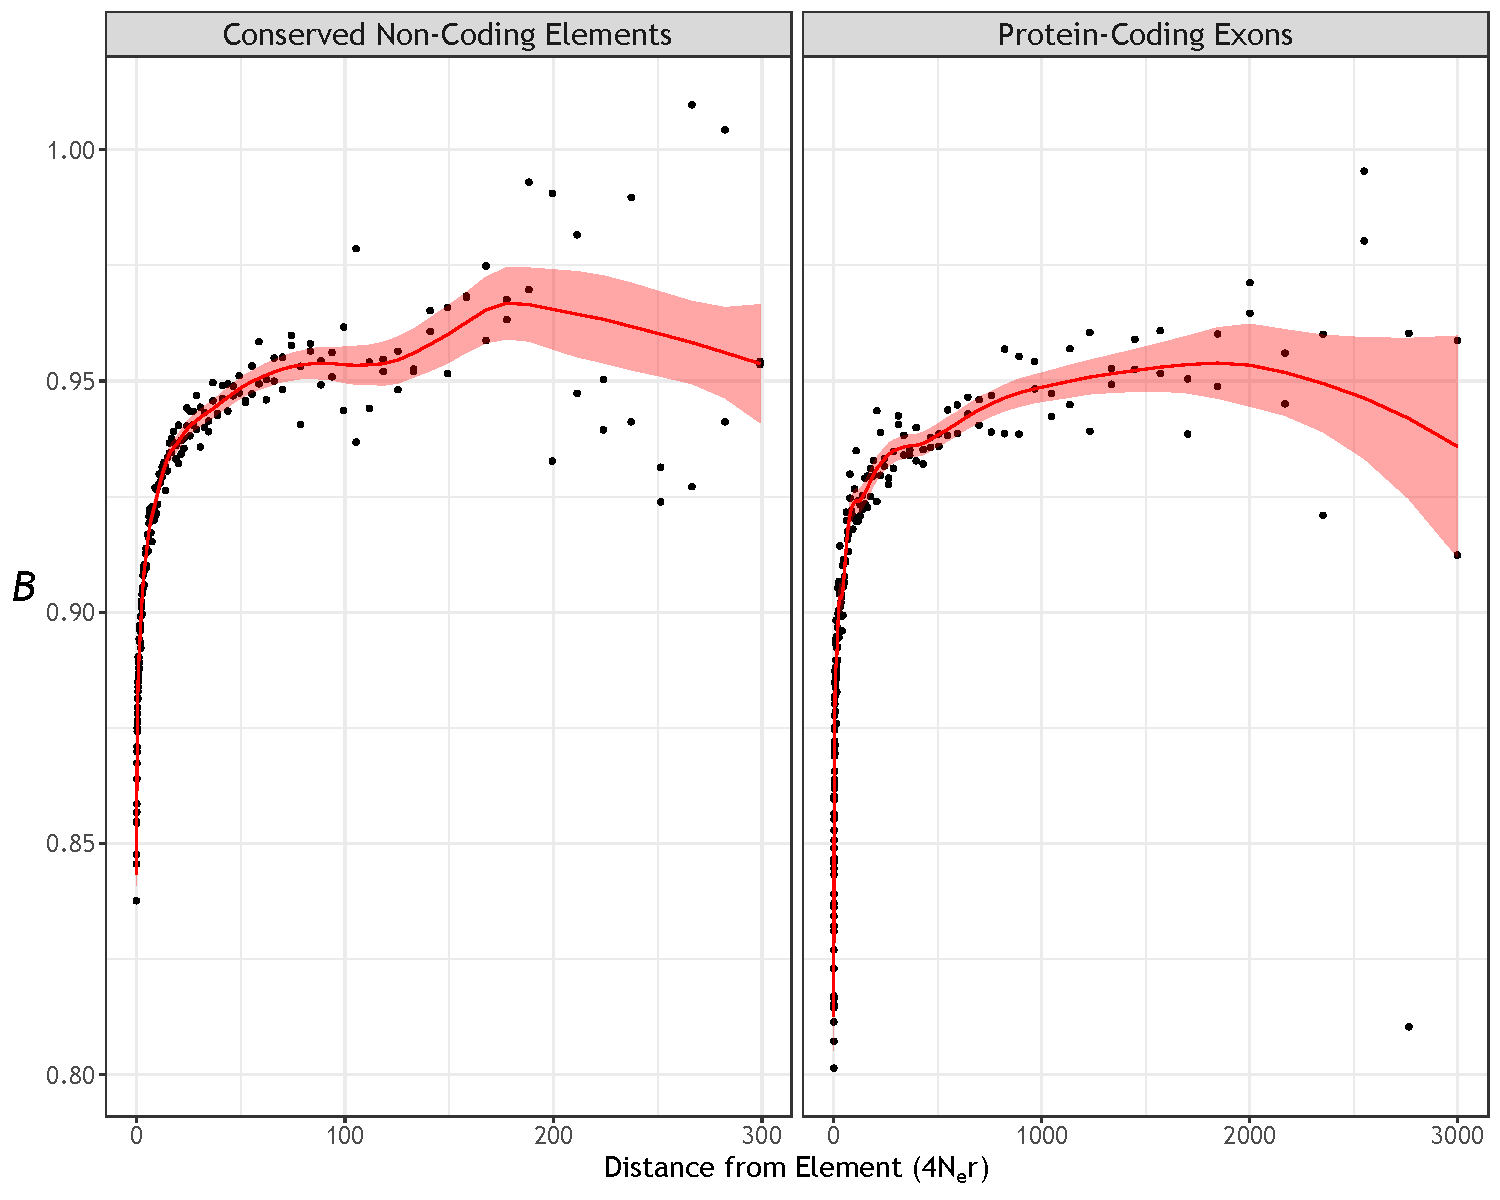
\includegraphics[width=\textwidth]{/Users/s0784966/PhD/Coding/Estimate_selection_from_troughs/BGS/BGSplotLoess.pdf}}
 \caption{Reductions in diversity around protein-coding exons and CNEs in simulations. Red lines are Loess curves fitted to the data with a span of 0.2, the ribbons are 95\% prediction intervals}.
 
 \label{fig:BGSLoess}
\end{figure}


\end{document}

\section*{junkyard}

Patterns of genetic diversity in a number of species are cons
In wild mice, there are troughs in diversity surrounding functional elements. In a recent analysis, we estimated the frequency and selection coefficients of advantageous mutations that occur in mice using distribution of derived allele frequencies (Booker and Keightley submitted). We showed that the parameters of selection obtained from the uSFS are unable to explain the patterns of selection observed in the genome.

Recently, Tataru \textit{et al.} (2017) showed that accurate estimates of positive election parameters an be obtained by analysis of the uSFS. However, the range of selection parameters that analysed may not

Recently, we have estimated the DFE using the uSFS for wild mice and shown that the parameters of selection that we infer do not explain the reductions in diversity observed around protein-coding exons. 


One of the long-standing goals of evolutionary biology has been to understand the contribution of coding versus non-coding change to adaptive evolution (King and Wilson; Carroll). Arguments have been made that regulatory regions, which may have a lower pleiotropic burden than protein-coding genes, may dominate phenotypic evolution. Indeed, regulatory regions are, on average,  subject to weaker selective constraints than protein-coding regions. In mice, 
In mice, there are reductions in genetic diversity around both conserved non-
Indeed, accurate estimates can be obtained even when ignoring between-species divergence (Table), as pointed out by Tataru \textit{et al} (2017). This is potentially very useful because divergence may bias parameter estimates if, for example, the DFE has changed  in the time since focal species and the outgroup(s) used to polarise alleles shared common ancestors.



	Strongly selected  In our simulations, we modelled cases where $gamma_a p_a$ = 0.05. This value
	 of $\gamma_a p_a$ is based on values estimated in studies of \textit{Drosophila melanogaster}. 
	
	In simulations incorporating strongly advantageous mutations (i.e. $gamma >$ 100), we found that positive selection could not be detected by analysis of polymorphism alone. Likelihood ratios between full DFE models and dDFE models fitted to the uSFS were not statistically significant when divergence was ignored (Table X). In such cases, advantageous mutations contribute little to standing variation, so there is little power to detect advantageous mutations from polymorphism alone. 
	
	Strongly selected, but rare advantageous mutations can be detected by analysis of the uSFS, if between-species divergence is included. data sets resulted in likelihood ratio tests, 
	This is evidenced by significant likelihood ratio tests for the presence of advantageous mutations. However, in these cases, the parameter values obtained are 
	 
	
	In such cases, advantageous mutations were detected when between-species did not substantially contribute to standing variation and so 
	

	
		Adaptive evolution was fairly frequent in our simulations ($\alpha$ $\approx30$\%), 
	ignoring the contribution of advantageous mutations to both standing variation and between-species divergence, either by modelling only the dDFE or by excluding divergence from calculations, led to biased parameter estimates, consistent with the findings of Tataru \textit{et al} (2017). 
	
	Estimates of the parameters of the dDFE were recovered from simulated populations with high precision. Our simulations assumed a gamma dDFE, but also included of advantageous mutations. When divergence was included in the iner
	Ignoring the contribution of advantageous mutations to the uSFS (i.e. by estimating only the dDFE parameters) resulted in dDFE parameter estimates that were substantially biased (Table SX). This was particularly 
	


	The strength and frequency of new advantageous mutations can be  estimated from both the uSFS and patterns of genetic diversity at linked sites. 

	In our simulaitons, we modelled strongly selected mutations at different frequencies. 
	
	When analysing simulation data we used the actual DFE model assumed in the simulations. This is obviously not possible when analysing real data, where the true nature of the DFE is unknown. Estimates of the DFE for harmful mutations obtained using uSFS analysis methods can be biased if positive selection is present but not modelled 
	
The fitness effects and 

When advantageous mutaitons are frequent, the product $\gamma p_a$ is accurately estimated fromt the uSFS. However, the individual parameters are difficult to disentangle. 
	
		

